\chapter{Scan Matching}
\label{sec:scan_matching}

\section{Overview of Scan Matching}

Scan matching refers to the process of finding a rigid transformation $T = \left( R \mid {\bf t} \right) \in {\rm SE}(3)$ that correctly aligns two point clouds.
Suppose we consider aligning two point clouds, $\mathcal{P} = ({\bf p}_{1}, \cdots, {\bf p}_{N})$ and $\mathcal{Q} = ({\bf q}_{1}, \cdots, {\bf q}_{M})$, where ${\bf p}, {\bf q} \in \mathbb{R}^{3}$.
In this case, we consider the following cost function\footnote{In implementation, the Huber loss shown in equation~(\ref{eq:huber_loss}) is employed. However, to avoid unnecessary complexity in the explanation, the Huber loss is omitted in this chapter.}.
%
\begin{align}
  E({\bf t}, R) = \sum_{i=1}^{N} \left\| {\bf q}_{i} - \left( R {\bf p}_{i} + {\bf t} \right) \right\|_{2}^{2},
  \label{eq:icp_cost_SO(3)}
\end{align}
%
where ${\bf q}_{i}$ denotes the point in $\mathcal{Q}$ that is closest to the transformed point $R {\bf p}_{i} + {\bf t}$.
To search for such nearest neighbors, data structures such as kd-trees are typically used.
In the implementation presented in this book, we employ the library {\it nanoflann}\footnote{\url{https://github.com/jlblancoc/nanoflann}}.

Equation~(\ref{eq:icp_cost_SO(3)}) can also be written as follows.
%
\begin{align}
  E(T) = \sum_{i=1}^{N} \left\| {\bf q}_{i} - T {\bf p}_{i} \right\|_{2}^{2}.
  \label{eq:icp_cost_SE(3)}
\end{align}
%
When expressed in the form of equation~(\ref{eq:icp_cost_SE(3)}), we have ${\bf p}, {\bf q} \in \mathbb{R}^{4}$, with the fourth element of each set to $1$.
Consequently, $T{\bf p}$ is also a four-dimensional vector with its fourth element equal to $1$.
Since the fourth element of ${\bf q}$ is likewise $1$, the fourth component of ${\bf q} - T{\bf p}$ is always zero.
As a result, the value of the cost function is identical to that given in equation~(\ref{eq:icp_cost_SO(3)}).
In the following, we define ${\bf r} = {\bf q} - T{\bf p}$ as the residual vector.

In scan matching, the goal is to estimate the rigid transformation shown below.
%
\begin{align}
  T^{*} = \argmin_{T} E(T).
  \label{eq:icp_scan_matching}
\end{align}
%
Equation~(\ref{eq:icp_scan_matching}) indicates that the goal is to find the pose $T^{*}$ that minimizes the cost function $E$.
Since $T^{*}$ is generally obtained through an iterative process, this method is referred to as {\bf Iterative Closest Point} (ICP) scan matching.
Note that scan matching that minimizes the cost defined in equation~(\ref{eq:icp_cost_SE(3)}) seeks to minimize the distances between corresponding points, and is therefore called point-to-point ICP.

However, point-to-point ICP is generally considered sensitive to noise.
For this reason, in this book we focus on point-to-plane ICP, which minimizes the distance between points and planes and is known to provide greater robustness.
In point-to-plane ICP, the following cost function is considered.
%
\begin{align}
  E(T) = \sum_{i=1}^{N} \left( {\bf n}_{i}^{\top} {\bf r}_{i} \right)^{2},
  \label{eq:point-to-plane_icp_cost_SE(3)}
\end{align}
%
where ${\bf n}_{i}$ denotes the normal vector in three-dimensional space, computed from the neighboring points of ${\bf q}_{i}$, and we define the residual as $r_{i} = {\bf n}_{i}^{\top} {\bf r}_{i}$.
These relationships are illustrated in Fig.~\ref{fig:normal_residual}.
Note that since ${\bf r}$ is a four-dimensional vector, ${\bf n}$ is also expressed as a four-dimensional vector.
However, because the fourth component of ${\bf r}$ is always zero, the value of the fourth component of ${\bf n}$ has no effect on the computation.

\begin{figure}[!t]
  \centering
  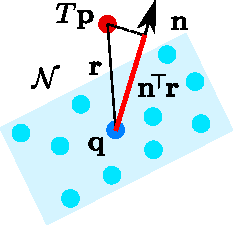
\includegraphics[width=0.2\textwidth]{../figs/normal_residual.pdf}
  \caption{Residual error used in point-to-plane ICP.}
  \label{fig:normal_residual}
\end{figure}

In the following, we first describe the method for computing the normal vectors, then derive the Jacobian associated with the residual vector, and finally explain how this Jacobian is used to perform optimization via the Gauss-Newton method.










\section{Computation of Normal Vectors}

To compute the normal vector at a point ${\bf q}$, we first collect the neighboring points around ${\bf q}$ and denote this set as $\mathcal{N}$.
Using this set, we then compute the mean $\bar{{\bf q}}$.
%
\begin{align}
  \bar{ {\bf q} } = \frac{1}{ | \mathcal{N} | } \sum_{ {\bf q}_{i} \in \mathcal{N} } {\bf q}_{i}.
  \label{eq:points_mean}
\end{align}
%
Next, we compute the covariance matrix $C$ of $\mathcal{N}$.
%
\begin{align}
  C = \frac{1}{ | \mathcal{N} | } \sum_{ {\bf q}_{i} \in \mathcal{N} } \left( {\bf q}_{i} - \bar{ {\bf q} } \right) \left( {\bf q}_{i} - \bar{ {\bf q} } \right)^{\top}.
  \label{eq:points_covariance}
\end{align}
%
Then, we perform eigen decomposition of $C$.
%
\begin{align}
  C = V \Lambda V^{\top},
\end{align}
%
where $V = \left( {\bf v}_{1} ~ {\bf v}_{2} ~ {\bf v}_{3} \right)$ and $\Lambda = {\rm diag} \left( \lambda_{1}, \lambda_{2}, \lambda_{3} \right)$, where ${\bf v}_{i}$ and $\lambda_{i}$ denote the eigenvectors and their corresponding eigenvalues, respectively.

The eigenvalues represent the variance of the points along each direction.
The eigenvector corresponding to the smallest eigenvalue indicates the direction with the least variance, i.e., the most compressed direction.
Therefore, when the smallest eigenvalue $\lambda_{\min}$ is sufficiently small, the corresponding eigenvector ${\bf v}_{\min}$ can be regarded as the normal vector of the local plane on which the points lie.
The vector ${\bf v}_{\min}$ obtained in this way is defined as the normal vector ${\bf n}$ at point ${\bf q}$.
Moreover, by setting a threshold on $\lambda_{\min}$, points with insufficient planarity can be excluded.










\section{Computation of the Jacobian}
\label{subsec:point_to_plane_jacobian}

In solving point-to-plane ICP using the Gauss-Newton method, we derive the Jacobian of the residual $r = {\bf n}^{\top} {\bf r}$ with respect to the pose $T$.
This Jacobian can be computed using the chain rule as follows.
%
\begin{align}
  \frac{ \partial r }{ \partial T } = \frac{ \partial r }{ \partial {\bf r} }
                                      \frac{ \partial {\bf r} }{ \partial T }.
\end{align}
%
Since $r = {\bf n}^{\top} {\bf r}$, it is clear that $\partial r / \partial {\bf r} = {\bf n}^{\top}$.
Therefore, in the following, we present the detailed computation only for $\partial {\bf r} / \partial T$.

The residual vector ${\bf r}$ is clearly a function of the pose $T$.
Thus, the Jacobian $J$ can be derived by considering the following expression.
%
\begin{align}
  {\bf r} \left( \exp \left( \delta \boldsymbol \xi^{\wedge} \right) T \right) - {\bf r} \left( T \right) =
  J \delta \boldsymbol \xi,
  \label{eq:point_plane_icp_jacob_approx}
\end{align}
%
where $\delta \boldsymbol{\xi}^{\wedge} = \left( \delta {\bf v}^{\top} ~ \delta \boldsymbol{\phi}^{\top} \right)^{\wedge} \in \mathfrak{se}(3)$, and $\exp \left( \delta \boldsymbol{\xi}^{\wedge} \right) T$ represents the state obtained by applying an infinitesimal perturbation to $T$ from the left in the space of ${\rm SE}(3)$.
Expanding the left-hand side of equation~(\ref{eq:point_plane_icp_jacob_approx}) yields the following.
%
\begin{align}
  \begin{split}
    {\bf q} - \exp \left( \delta \boldsymbol \xi^{\wedge} \right) T {\bf p} - \left( {\bf q} - T {\bf p} \right)
    %
    = & - \left( \exp \left( \delta \boldsymbol \xi^{\wedge} \right) - I_{4} \right) T {\bf p}, \\
    %
    = & - \left( \left( \begin{matrix} I_{3} + \delta \boldsymbol \phi^{\wedge} & \delta {\bf v} \\ {\bf 0}^{\top} & 1 \end{matrix} \right) - I_{4} \right) \left( \begin{matrix} R {\bf p} + {\bf t} \\ 1 \end{matrix} \right), \\
    %
    = & - \left( \begin{matrix} \delta \boldsymbol \phi^{\wedge} & \delta {\bf v} \\ {\bf 0}^{\top} & 0 \end{matrix} \right) \left( \begin{matrix} {\bf p}^{'} \\ 1 \end{matrix} \right), \\
    %
     = & - \left( \begin{matrix} \delta \boldsymbol \phi^{\wedge} {\bf p}^{'} + \delta {\bf v} \\ 0 \end{matrix} \right), \\
    %
     = & \left( \begin{matrix} \left( {\bf p}^{'} \right)^{\wedge} \delta \boldsymbol \phi - \delta {\bf v} \\ 0 \end{matrix} \right), \\
     %
     = & \left( \begin{matrix} -I_{3} & \left( {\bf p}^{'} \right)^{\wedge} \\ {\bf 0}^{\top} & {\bf 0}^{\top} \end{matrix} \right) \delta \boldsymbol \xi,
  \end{split}
\end{align}
%
where we set ${\bf p}^{'} = R{\bf p} + {\bf t}$ and use the relation $\delta \boldsymbol{\phi}^{\wedge} {\bf p}^{'} = -\left( {\bf p}^{'} \right)^{\wedge} \delta \boldsymbol{\phi}$.
Therefore, the Jacobian with respect to the residual is given as follows.
%
\begin{align}
  \begin{split}
    \frac{ \partial r }{ \partial T } = & {\bf n}^{\top} \left( \begin{matrix} -I_{3} & \left( {\bf p}^{'} \right)^{\wedge} \\ {\bf 0}^{\top} & {\bf 0}^{\top} \end{matrix} \right), \\
    %
    = & \left( \begin{matrix} -{\bf n}^{\top} & {\bf n}^{\top} \left( {\bf p}^{'} \right)^{\wedge} \end{matrix} \right) \in \mathbb{R}^{1 \times 6}.
  \end{split}
  \label{eq:point_to_plane_icp_jacobian}
\end{align}
%
Note that the final ${\bf n} \in \mathbb{R}^{3}$ represents the three-dimensional normal vector.













\section{Optimization Using the Gauss-Newton Method}

Using the Jacobian given in equation~(\ref{eq:point_to_plane_icp_jacobian}), the Hessian matrix and gradient vector for solving point-to-plane ICP scan matching with the Gauss-Newton method are obtained as follows.
%
\begin{align}
  \begin{gathered}
    H = \sum_{i=1}^{N} J_{i}^{\top} J_{i}, \\
    {\bf b} = \sum_{i=1}^{N} J_{i}^{\top} r_{i}. 
  \end{gathered}
  \label{eq:point_to_plane_icp_hessian_and_gradient}
\end{align}
%
When using the Huber loss, we define $w_{i} = \rho^{\prime}\left( r_{i}^{2} \right)$ based on equation~(\ref{eq:huber_loss_prime}), and compute $H = \sum_{i} w_{i} J_{i}^{\top} J_{i}$ and ${\bf b} = \sum_{i} w_{i} J_{i}^{\top} r_{i}$.
Then, using $H$ and ${\bf b}$ as defined in equation~(\ref{eq:point_to_plane_icp_hessian_and_gradient}), we solve for $\delta \boldsymbol{\xi}$ such that $H \delta \boldsymbol{\xi} = -{\bf b}$.
Finally, the state is updated as follows.
%
\begin{align}
  T \leftarrow \exp \left( \delta \boldsymbol \xi^{\wedge} \right) T.
\end{align}
%
This update is repeated until either $\| \delta \boldsymbol{\xi} \|_{2} \leq \epsilon$ or a predefined number of iterations is reached, at which point $T^{*}$ in equation~(\ref{eq:icp_scan_matching}) is considered to have been obtained.
Here, $\epsilon$ is an arbitrary constant.












\section{Practical Considerations}
\label{sec:scan_matching_実用にあたって}

To execute scan matching accurately, obtaining a good initial estimate is of critical importance.
If the initial estimate is sufficiently accurate, correspondence search operates reliably, and scan matching converges to the optimal solution with high precision.
Conversely, if the initial estimate contains large errors, correspondence search is likely to fail, causing scan matching to break down.
It should also be noted that scan matching may converge to a solution that does not minimize the cost function; such solutions are referred to as {\bf local minima}.

To mitigate the effects of incorrect correspondences, it is effective to introduce a robust kernel such as the Huber loss.
By suppressing the influence of large residuals, the Huber loss can prevent optimization from being significantly degraded by outliers.
However, the Huber loss is not a universal remedy.
For instance, when a small number of correct correspondences are mixed with a large number of incorrect ones, the residuals of the correct correspondences may still be large.
In such cases, the Huber loss reduces their weights as well, leading to an underestimation of their contribution.
As a result, scan matching may succeed without the Huber loss but fail when it is applied.
Therefore, the parameter $\delta$ of the Huber loss must be carefully tuned.
Nevertheless, in most cases, introducing the Huber loss improves the robustness of scan matching.

It is also difficult for scan matching alone to provide a reliable initial estimate at every frame, particularly when the motion involves high translation or rotation speeds.
To address this issue, it is effective to integrate external sensors such as IMUs, which can provide more accurate initial estimates.
In the next chapter, we discuss a method for loosely coupling LiDAR and IMU measurements.

In addition to the initial estimate, attention must also be paid to the environment in which scan matching is performed.
Since scan matching determines rigid transformations based on geometric constraints, obtaining the correct solution requires an environment that provides sufficient constraints.
If appropriate constraints cannot be obtained, solving the Gauss-Newton equations $H \delta \boldsymbol{\xi} = -{\bf b}$ may fail to yield a valid $\delta \boldsymbol{\xi}$.
This occurs because $H$ becomes non-invertible, and its inverse cannot be defined.
Such cases are referred to as {\bf degeneracy}, in which scan matching fundamentally fails to function.
A common method to detect degeneracy is to perform eigenvalue decomposition of the Hessian matrix defined in equation~(\ref{eq:point_to_plane_icp_hessian_and_gradient}) and examine its smallest eigenvalue.
If the smallest eigenvalue is extremely small, the Hessian matrix becomes rank-deficient, preventing computation of a valid inverse.
Consequently, the optimization process breaks down.


